\section{有限长度纵向 PEEC}
\label{chapter:06}

% block-id: 06.peec_method.heading
\hypertarget{06.peec_method.heading}{}
\subsection{有限长度纵向 PEEC}

% block-id: 06.peec_method.p1
\hypertarget{06.peec_method.p1}{}
纵向 PEEC 将导体截面离散为体积细丝，每条细丝内采用沿轴向、沿长度均匀的复电流密度。欧姆电阻与有限体积对的部分电感由 \eqref{eq:E08} 给出，并形成 Z=R+jωL，随后按 \eqref{eq:E04} 施加公共端口和总电流约束。1264 与 5024 表示体积细丝自由度；这些细丝是连续导体的离散单元。同一截面内各体积细丝的电流差异表示内部电流集中，所用基函数的范围为纵向电流。

% block-id: 06.peec_method.p2
\hypertarget{06.peec_method.p2}{}
纵向算例的名义圆线直径为 2 mm。m40 与 m80 的方形细丝宽度分别为 0.050 mm 和 0.025 mm，对应实际截面面积 3.16 mm² 和 3.14 mm²。敏感性试验分别改变长度、互项积分或自项积分设置。1264 自由度模型采用同一截面与 0.16、0.32、0.64 m 三档长度；固定长度后，将互项积分阶数 q 依次取为 4、6、8，自项精度从 10/8 提高至 12/10；两个数字依次表示自项数值积分的 AccuracyGoal 与 PrecisionGoal，即绝对精度和相对精度的目标位数。5024 自由度模型复核 0.32、0.64 m 长度及相同积分变化。两种截面离散的铜面积略有差异，因此各档电阻分别与自身等面积圆线的 Bessel 解比较；跨档变化同时包含离散和面积近似的影响。

% block-id: 06.peec_method.p3
\hypertarget{06.peec_method.p3}{}
部分电感核包含有限导体周围的磁耦合，圆线 Bessel 解给出长直导体的内部阻抗。两者在本文中以耗散分量 Rac 进行比较，同时保留长度和面积条件。长度试验衡量当前核与纵向基函数的敏感性；横向环流、曲线股线和真实端部电流重分布需通过扩展自由度研究。与 FEM–PEEC 耦合方法 \cite{P03} 的联系在于场路联合描述，具体的激励、回流和场反馈方式仍应按各实现分别比较。

% block-id: 06.peec_derivation.heading
\hypertarget{06.peec_derivation.heading}{}
\subsection{纵向细丝基函数与核积分}

% block-id: 06.peec_derivation.p1
\hypertarget{06.peec_derivation.p1}{}
第 α 条体积细丝中的电流密度取为常量 iα/Aα，方向沿轴向。由矢势体积积分得到测试细丝内的感应电场，再沿长度积分，可得对称部分电感矩阵。自项在重合点具有可积奇性，使用专门的自项精度控制；互项采用独立积分阶数。欧姆电阻与 jωL 组成耦合矩阵，并与公共端电压和总电流约束联合求解。所用基函数决定了这一模型能够表示的电流方向。

% block-id: 06.peec_results.heading
\hypertarget{06.peec_results.heading}{}
\subsection{纵向 PEEC 的长度和积分敏感性}

% block-id: 06.peec_results.p1
\hypertarget{06.peec_results.p1}{}
1264 自由度模型在 0.16、0.32、0.64 m 的电阻分别为 19.8992、19.9586、19.9885 mΩ/轴向m，相邻长度变化为 0.298640\% 和 0.149482\%；5024 自由度模型的 0.32\(\to\)0.64 m 变化为 0.148730\%，见 图~\ref{fig:peec_length}。长度增加时电阻变化减小，且已检查增量均低于 1\%。该序列给出了 0.16–0.64 m 范围内的敏感性。

% block-id: 06.peec_results.p2
\hypertarget{06.peec_results.p2}{}
在 5024 自由度、Lz=0.64 m、互项 q=4、自项 12/10 时，Rac=\metric{peec_rac} mΩ/轴向m，Rac/Rdc=3.64472，损耗为 8.00510 W/轴向m，与该档等面积 Bessel 参照相差 0.044582\%。图~\ref{fig:peec_cross_section} 以保存的细丝电流和方形单元恢复截面电流分布，呈现导体内部的表层集中。这里的自由度属于连续导体离散，电流离散程度与前述绝缘股线间的均流指标具有不同含义。

% block-id: 06.peec_results.p3
\hypertarget{06.peec_results.p3}{}
互项 q=4\(\to\)6\(\to\)8、自项 10/8\(\to\)12/10 的结果见 图~\ref{fig:peec_sensitivity}。两种规模中，互项变化所对应的最大电阻相对变化为 1.21×10⁻⁵，最大复电流相对变化为 1.60×10⁻⁵；自项变化的相应最大值为 6.75×10⁻¹¹ 和 7.10×10⁻¹¹。横向粗细离散在 0.32、0.64 m 下的电阻变化分别为 0.122127\% 和 0.121376\%，该比较同时涉及实际面积变化。由此，积分设置的影响在当前试验中小于长度和截面离散的影响。解析参照与敏感性结果共同支持纵向模型的电阻计算，真实端区及横向电流的误差仍属于模型层面的研究问题。

% block-id: 06.equation.E08
\hypertarget{06.equation.E08}{}
\hypertarget{E08}{}
\begin{equation}
\begin{gathered}
R_{\alpha\beta}=\delta_{\alpha\beta}\frac{L_z}{\sigma A_\alpha} \\
L_{\alpha\beta}=\frac{\mu}{4\pi A_\alpha A_\beta}\int_{V_\alpha}\int_{V_\beta}\frac{\hat{\mathbf t}_\alpha\cdot\hat{\mathbf t}_\beta}{|\mathbf r-\mathbf r'|}\,\mathrm dV\,\mathrm dV'
\end{gathered}
\tag{7}\label{eq:E08}
\end{equation}

% block-id: 06.figure.peec_cross_section
\hypertarget{06.figure.peec_cross_section}{}
\begin{figure}[!htbp]
\centering
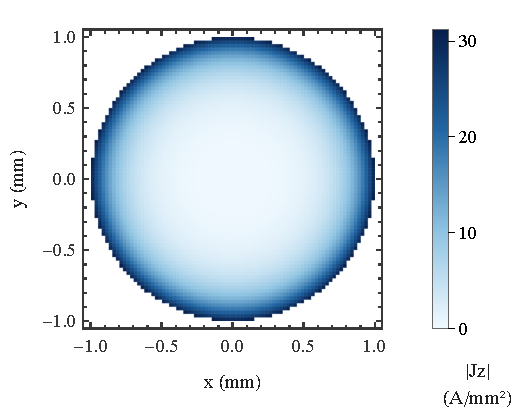
\includegraphics[width=\linewidth,height=.72\textheight,keepaspectratio]{../../assets/zh-CN/peec_cross_section.pdf}
\caption{纵向 PEEC 截面电流。 方形细丝单元的复电流恢复 RMS 幅值。 代表模型含 5024 条纵向体积细丝，轴向长度 0.64 m。坐标和材料面积采用该档实际方形离散定义。}
\label{fig:peec_cross_section}
\end{figure}

% block-id: 06.figure.peec_length
\hypertarget{06.figure.peec_length}{}
\begin{figure}[!htbp]
\centering
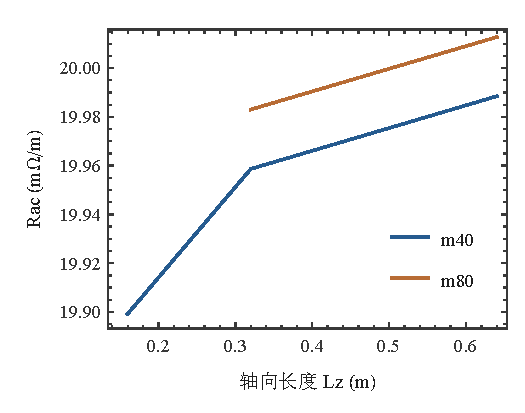
\includegraphics[width=\linewidth,height=.72\textheight,keepaspectratio]{../../assets/zh-CN/peec_length.pdf}
\caption{纵向 PEEC 长度敏感性。 同一截面按保存的轴向长度比较单位长度电阻。 1264 自由度模型采用 0.16、0.32、0.64 m，5024 自由度复核末两档。积分参数在每个长度序列内固定。}
\label{fig:peec_length}
\end{figure}

% block-id: 06.figure.peec_sensitivity
\hypertarget{06.figure.peec_sensitivity}{}
\begin{figure}[!htbp]
\centering
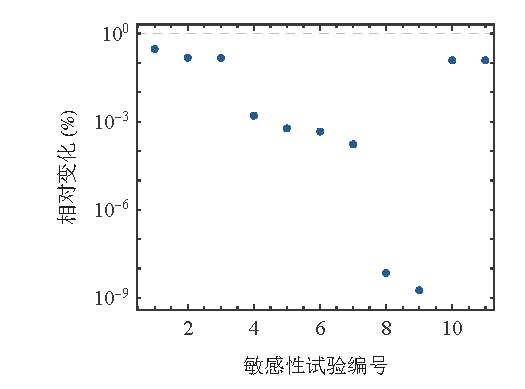
\includegraphics[width=\linewidth,height=.72\textheight,keepaspectratio]{../../assets/zh-CN/peec_sensitivity.pdf}
\caption{纵向 PEEC 积分敏感性。 互项阶数与自项精度各自进行单因素对照。 互项使用 q4、q6、q8，自项使用 10/8 与 12/10。比较保留同一截面及轴向长度。}
\label{fig:peec_sensitivity}
\end{figure}
